\documentclass[11pt]{article}
\usepackage{amsmath}
\usepackage{amsfonts}
\usepackage[]{graphicx}
\usepackage{subfig}
\begin{document}
%\maketitle

\begin{figure}[ht]
\centering
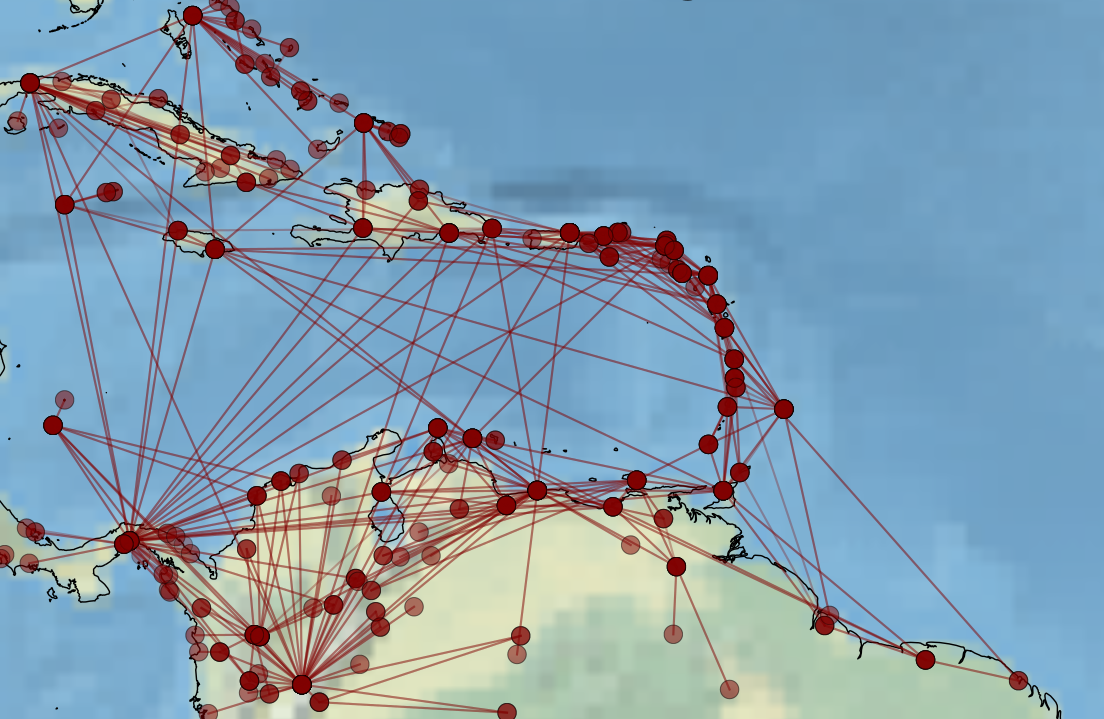
\includegraphics[scale=.17]{./caribbean_region}
\hspace{.8cm}
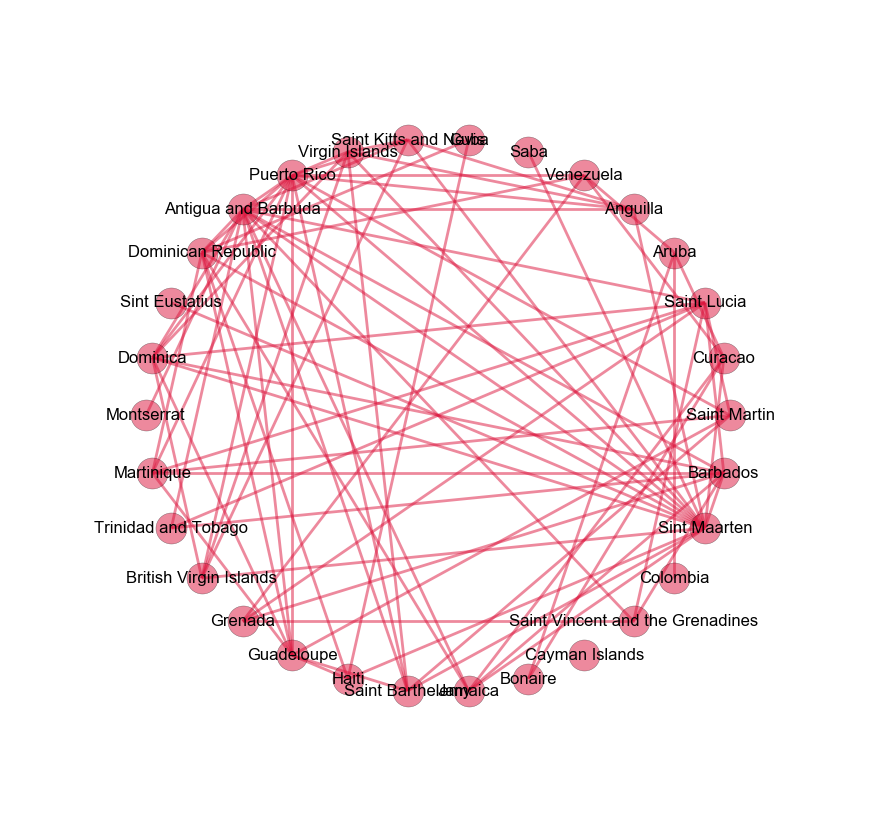
\includegraphics[scale=.16]{./simple_network_model_circular_and_labels_red_scen_A}\\
\caption{\small .}
\label{fig:map-and-network}
\end{figure}

\vspace{2cm}

\begin{figure}[ht]
\centering
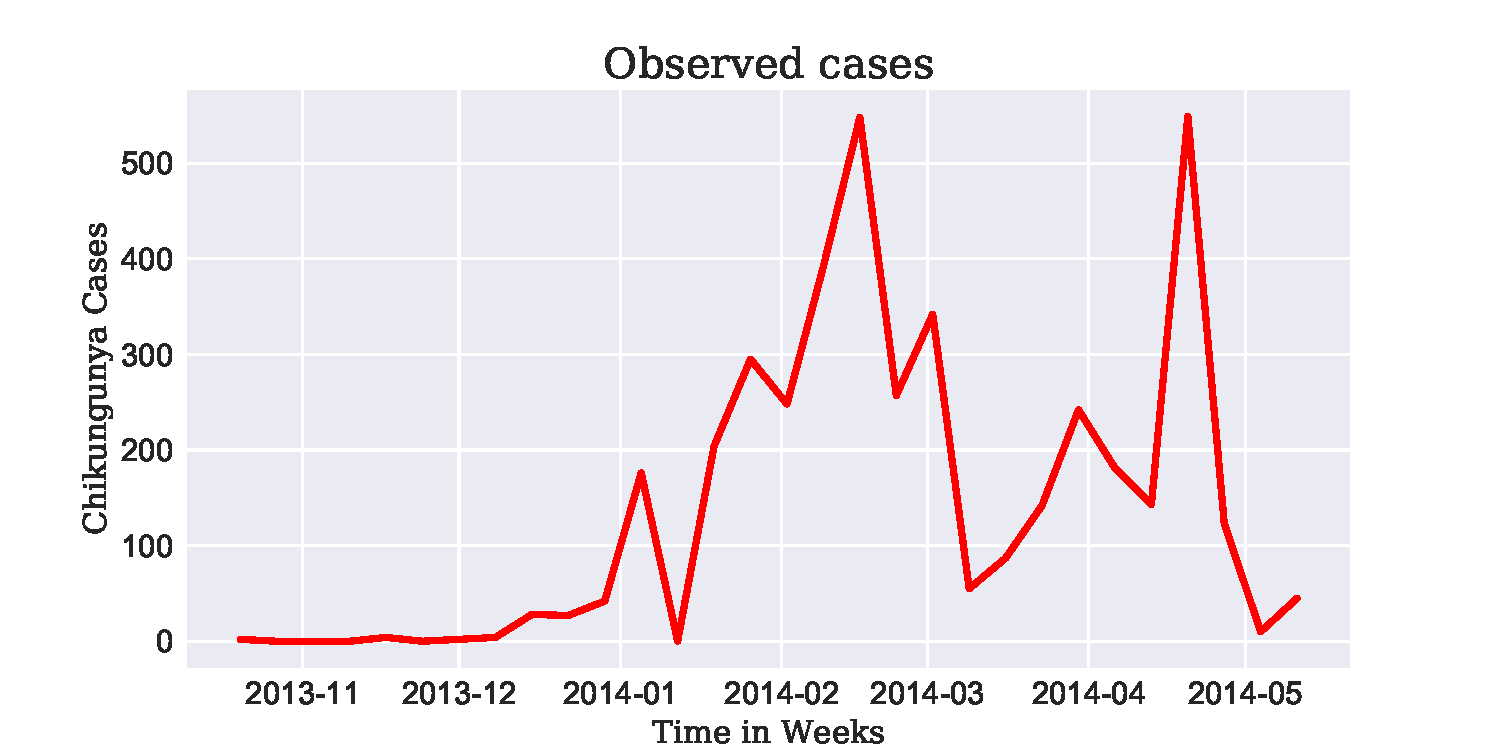
\includegraphics[scale=.23]{./observed_cases_st}
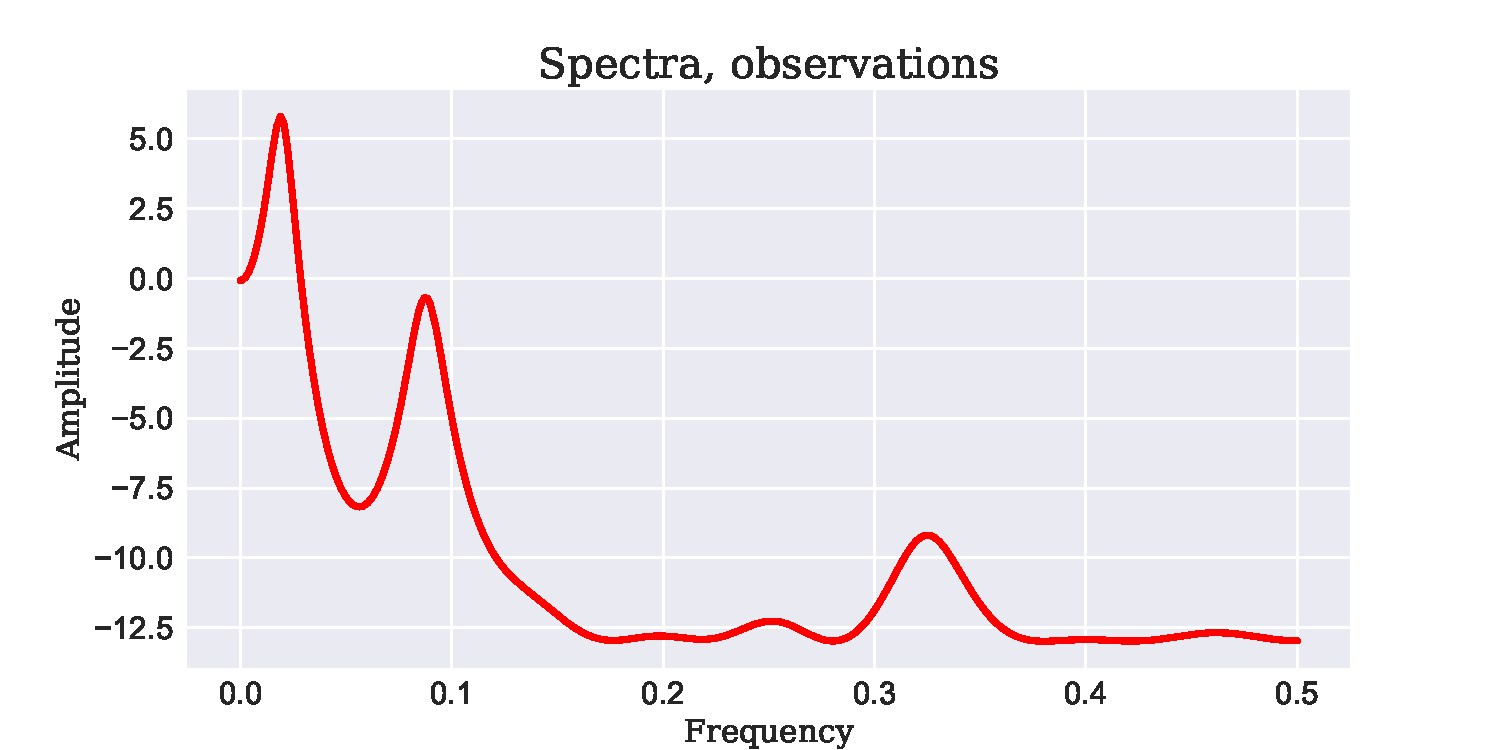
\includegraphics[scale=.23]{./spectra_obs}
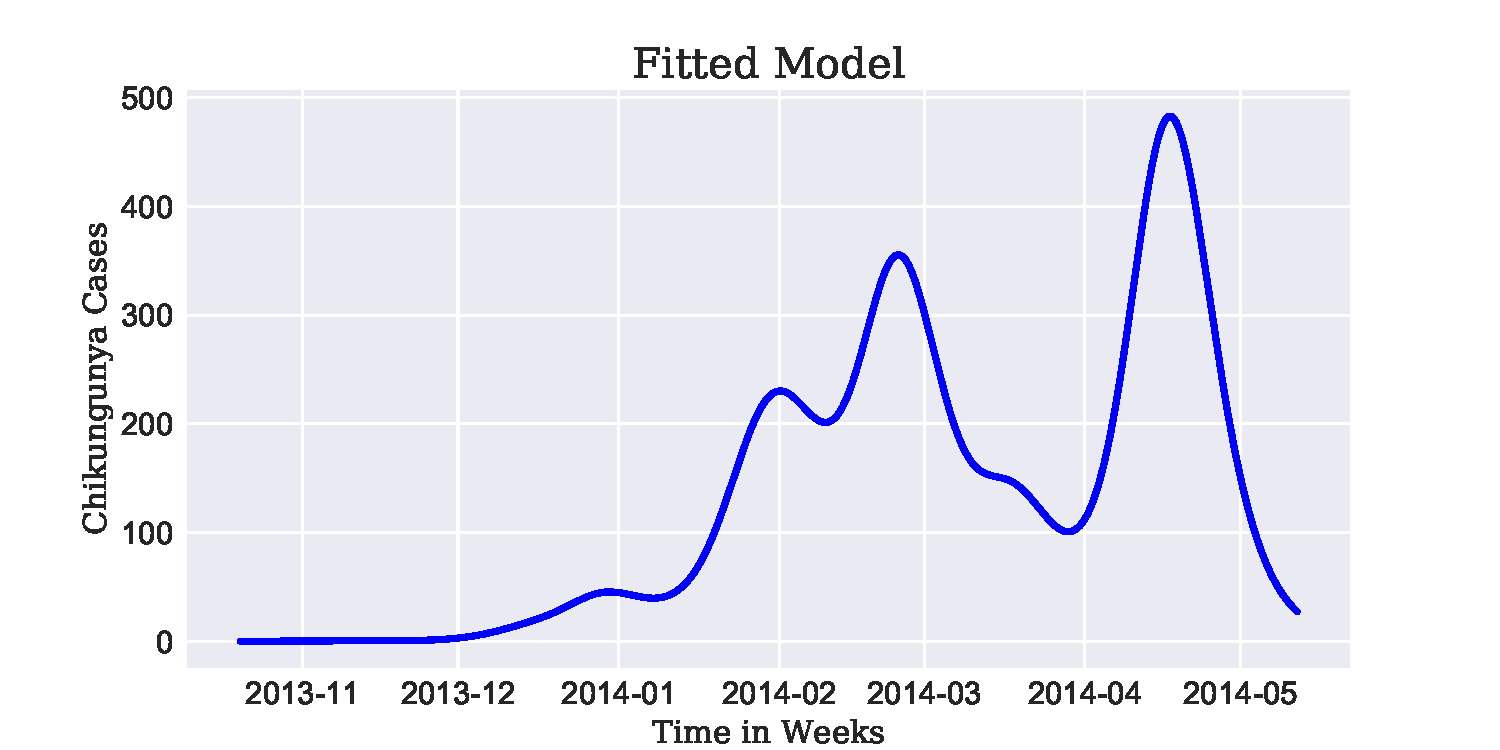
\includegraphics[scale=.23]{./fitted_model_st}
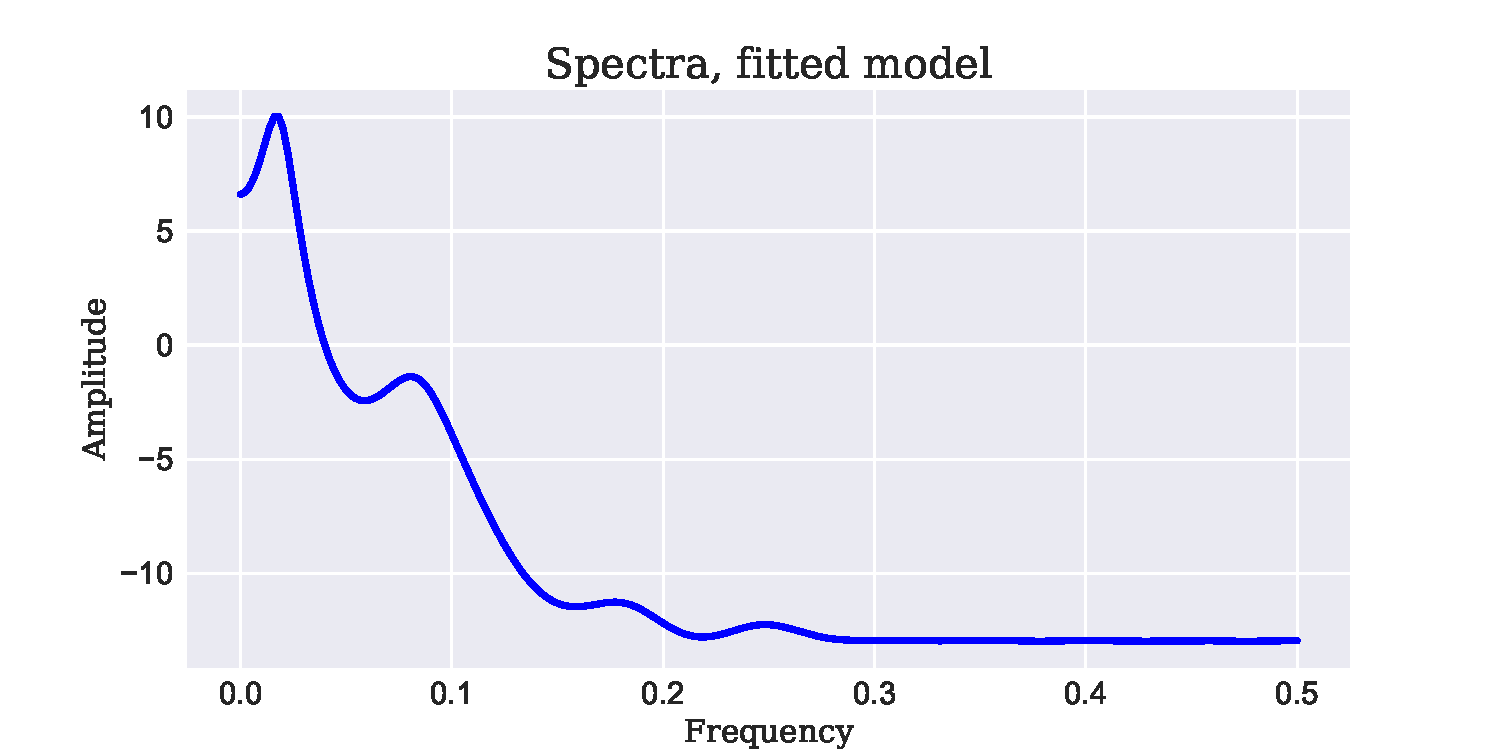
\includegraphics[scale=.23]{./spectra_sim}\\
\caption{\small .}
\label{fig:map-and-network}
\end{figure}

\vspace{2cm}

\begin{figure}[ht]
\centering
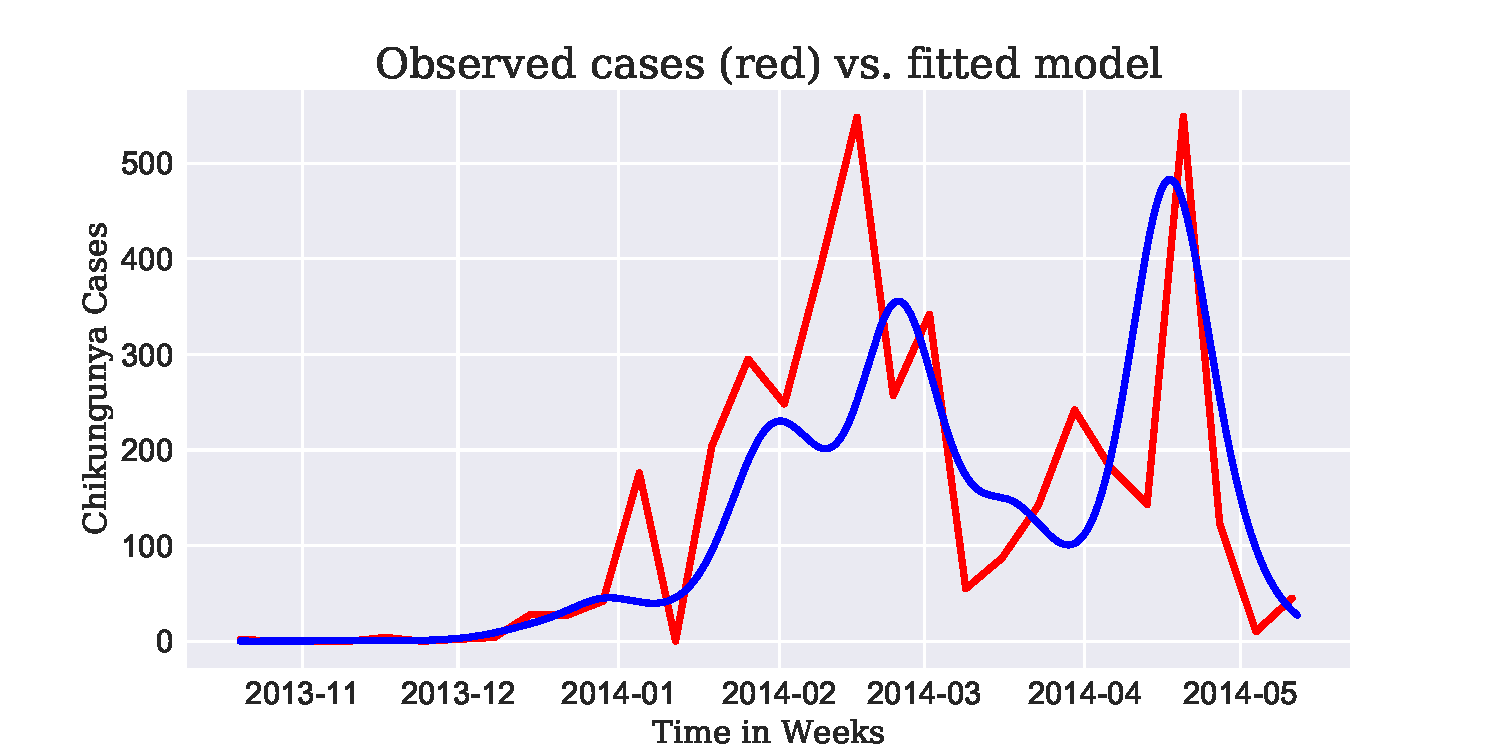
\includegraphics[scale=.23]{./observed_vs_fitted_st}
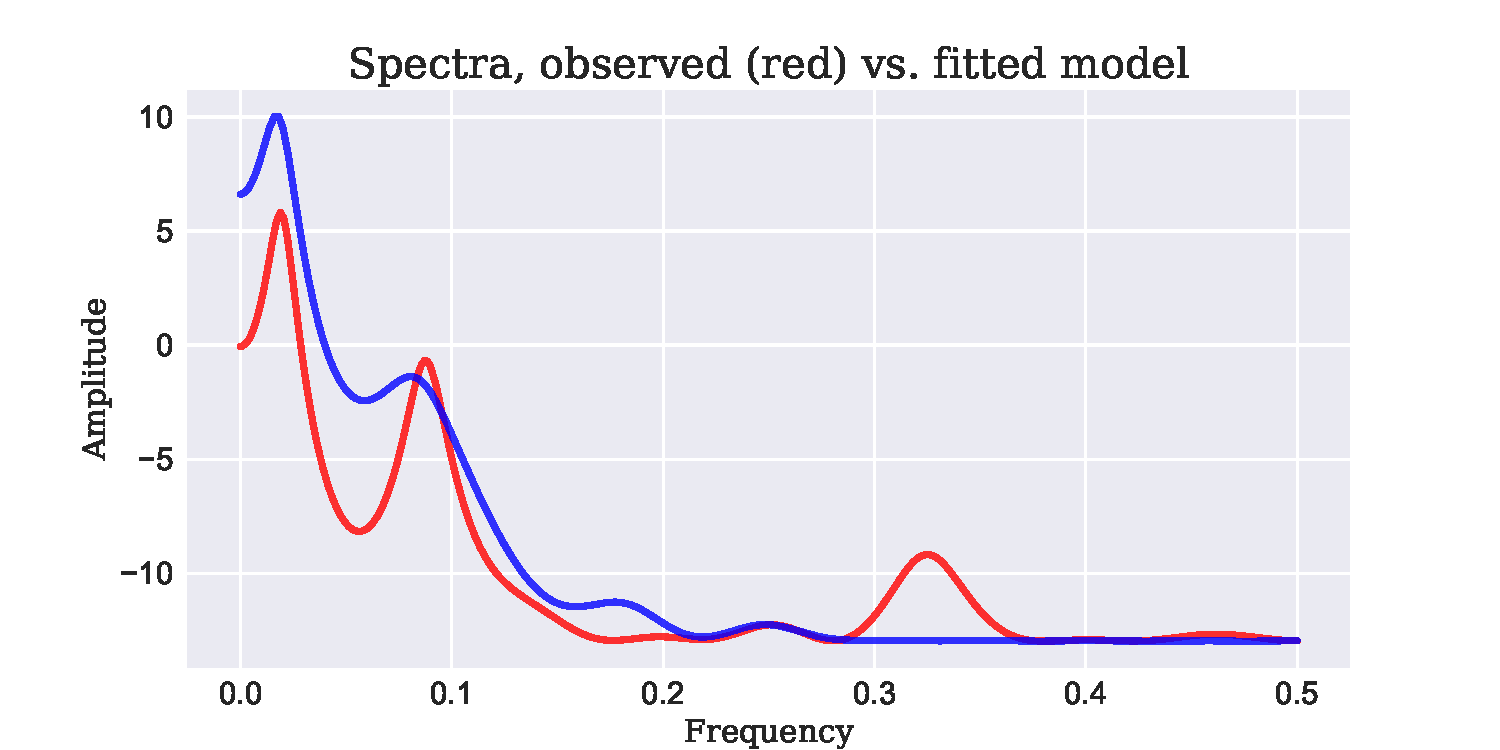
\includegraphics[scale=.23]{./spectra_obs_vs_sim}
\caption{\small . (optional for previous figure)}
\label{fig:map-and-network}
\end{figure}
%
\vspace{4cm}
%
\begin{figure}[ht]
\centering
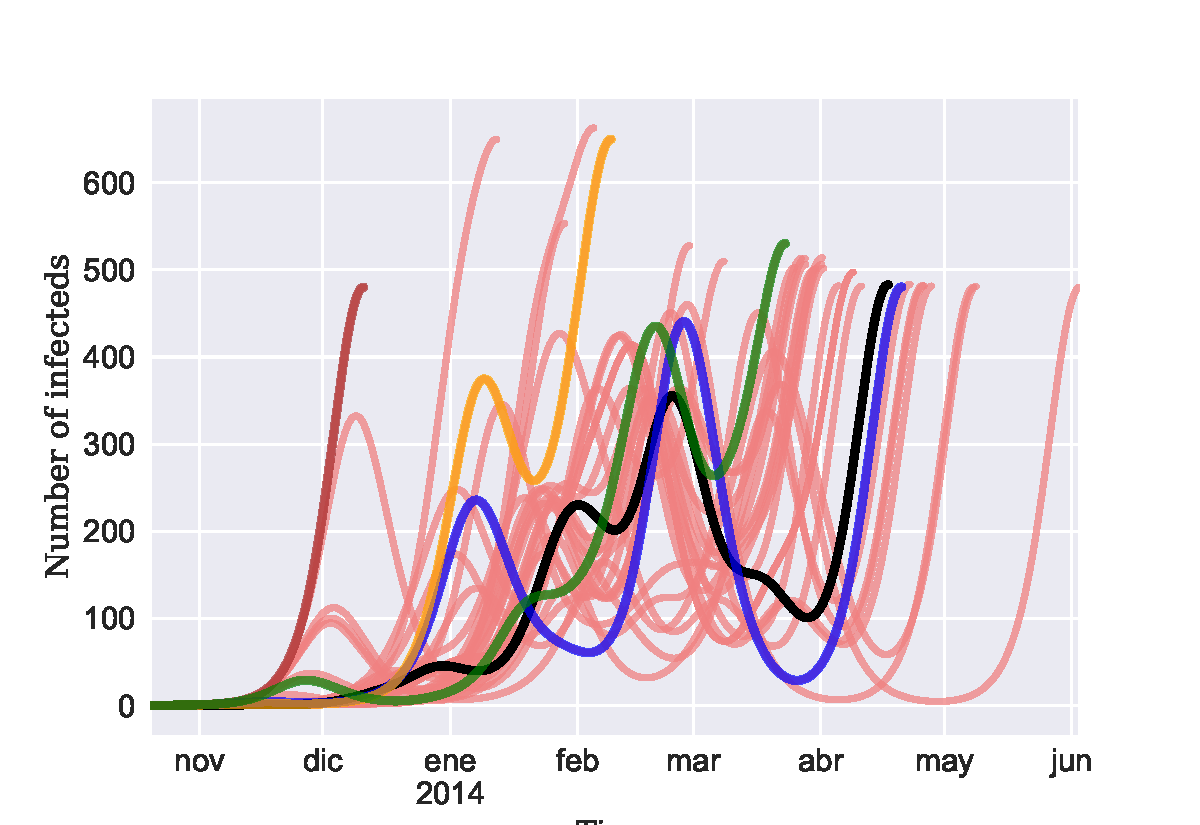
\includegraphics[scale=.35]{./scenario4_scenarioB}
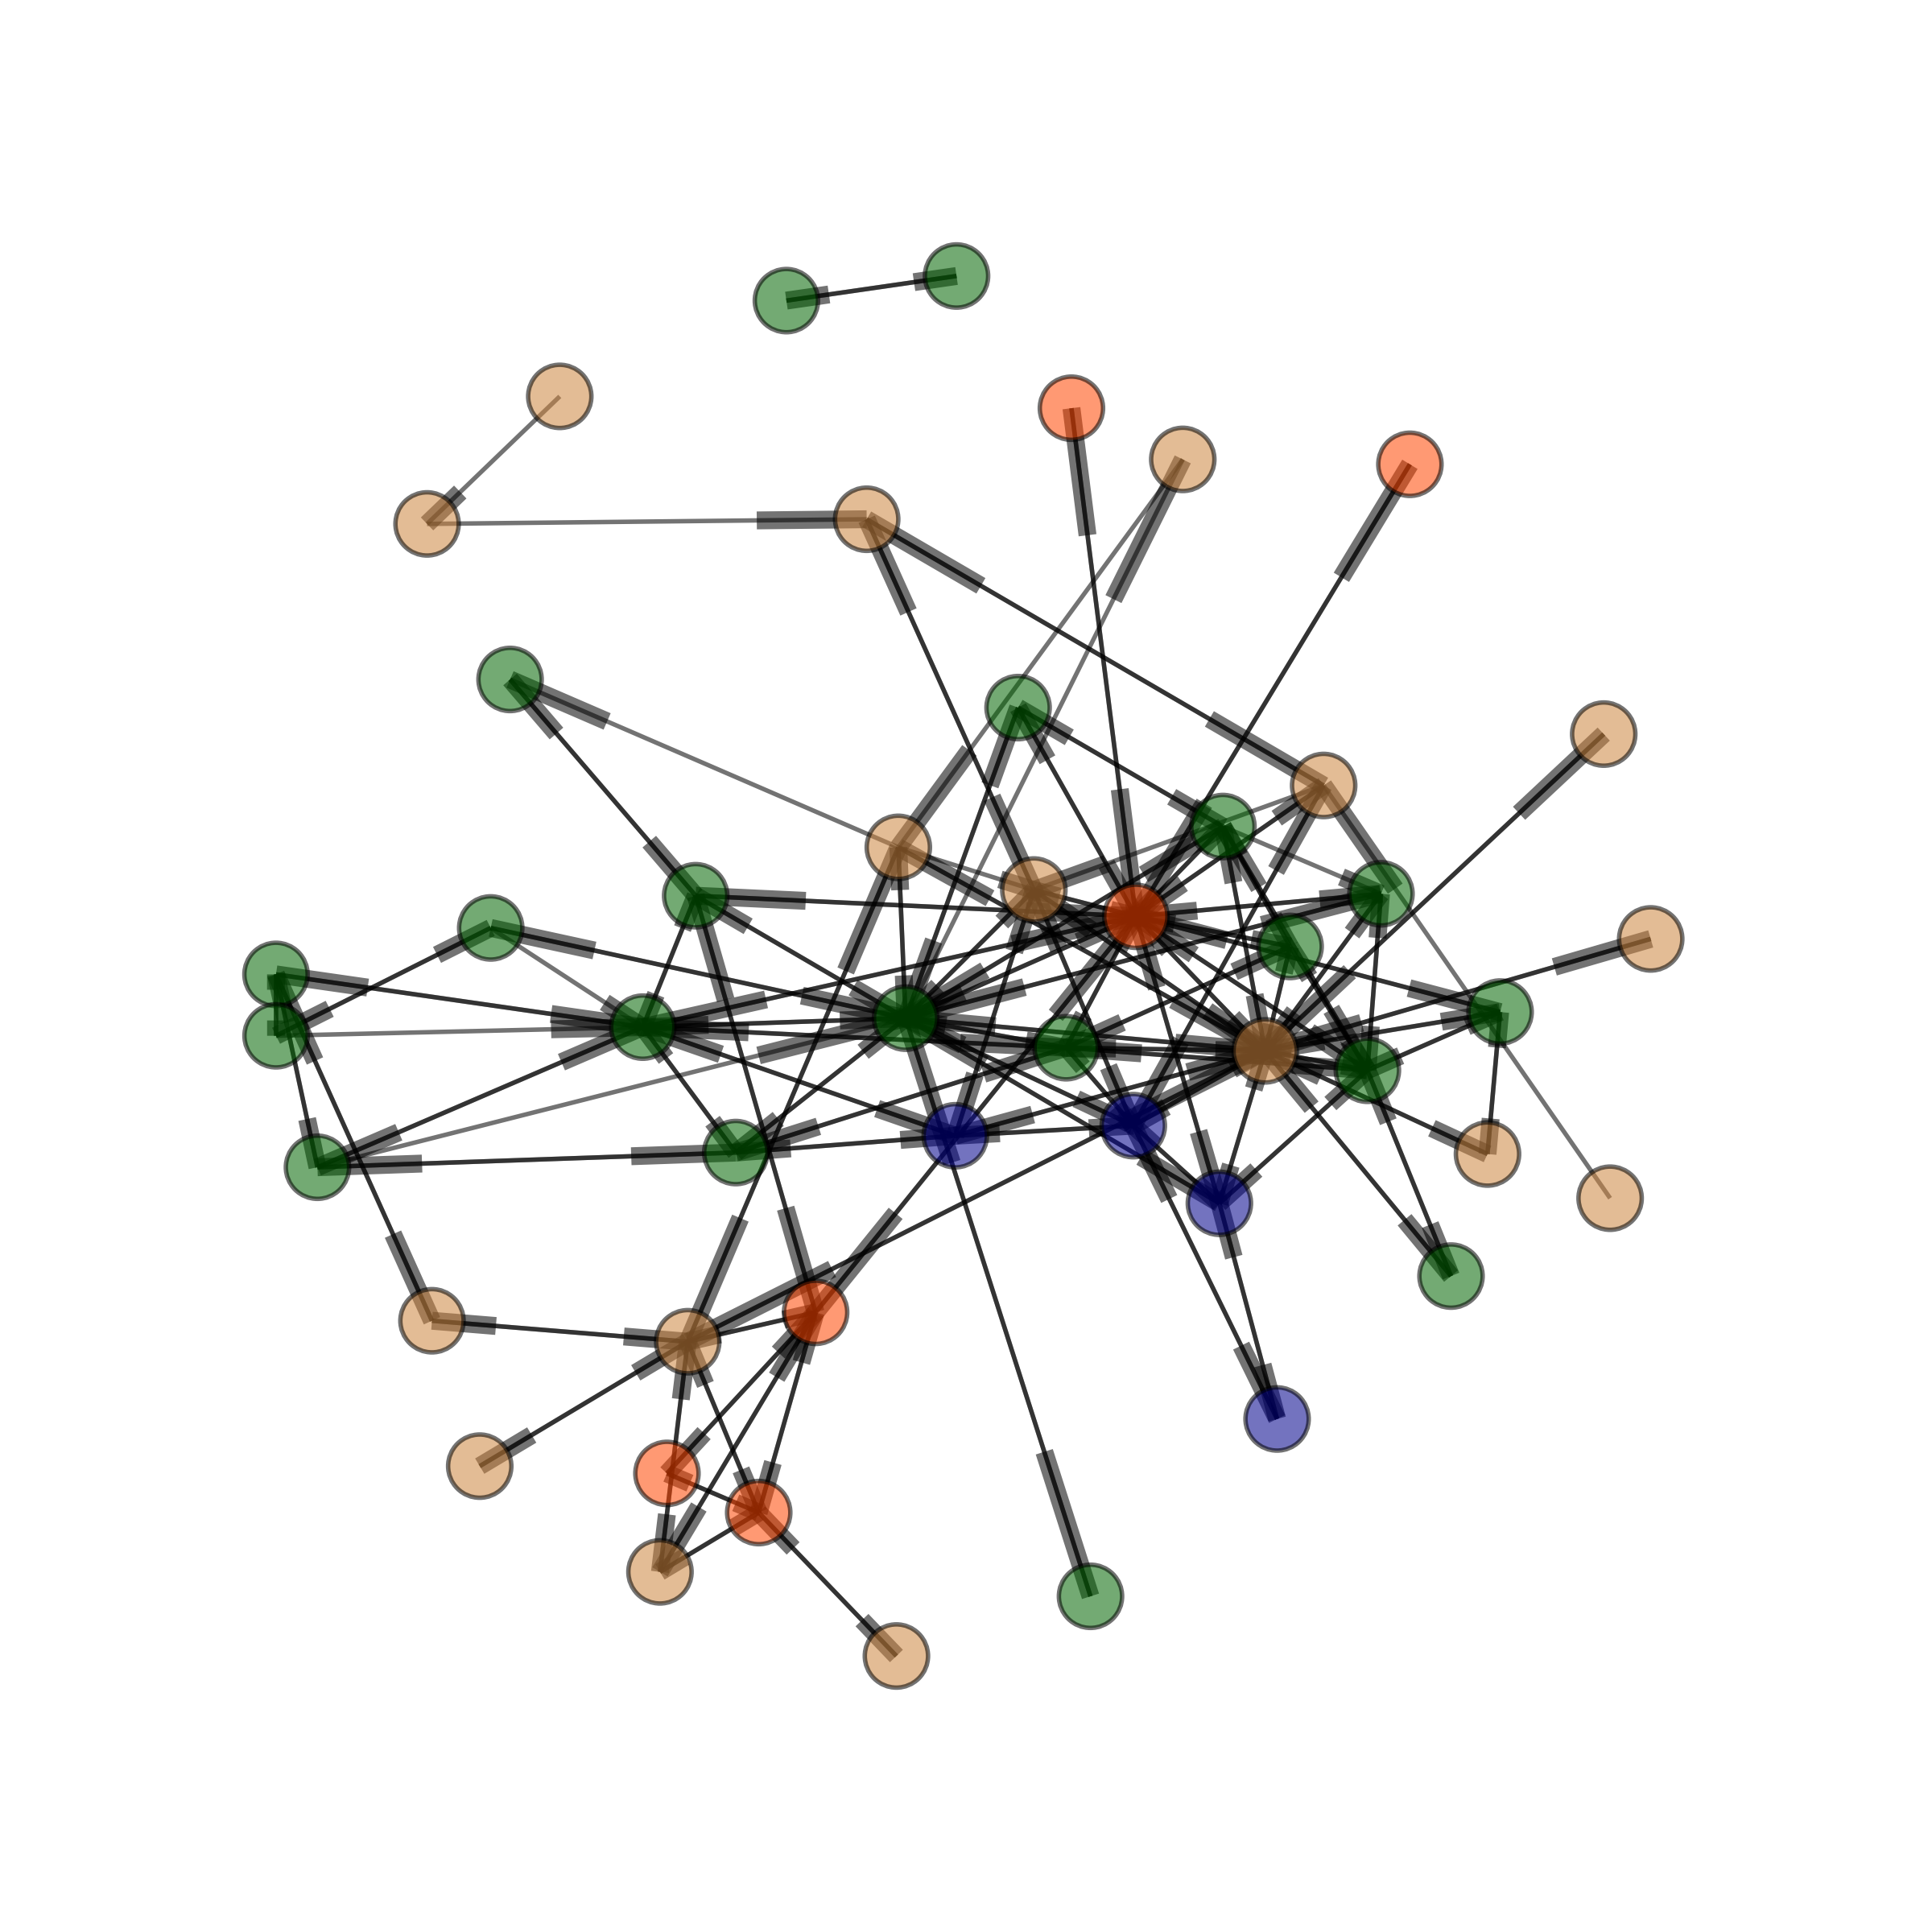
\includegraphics[scale=.30]{./graph_region3_colored}//
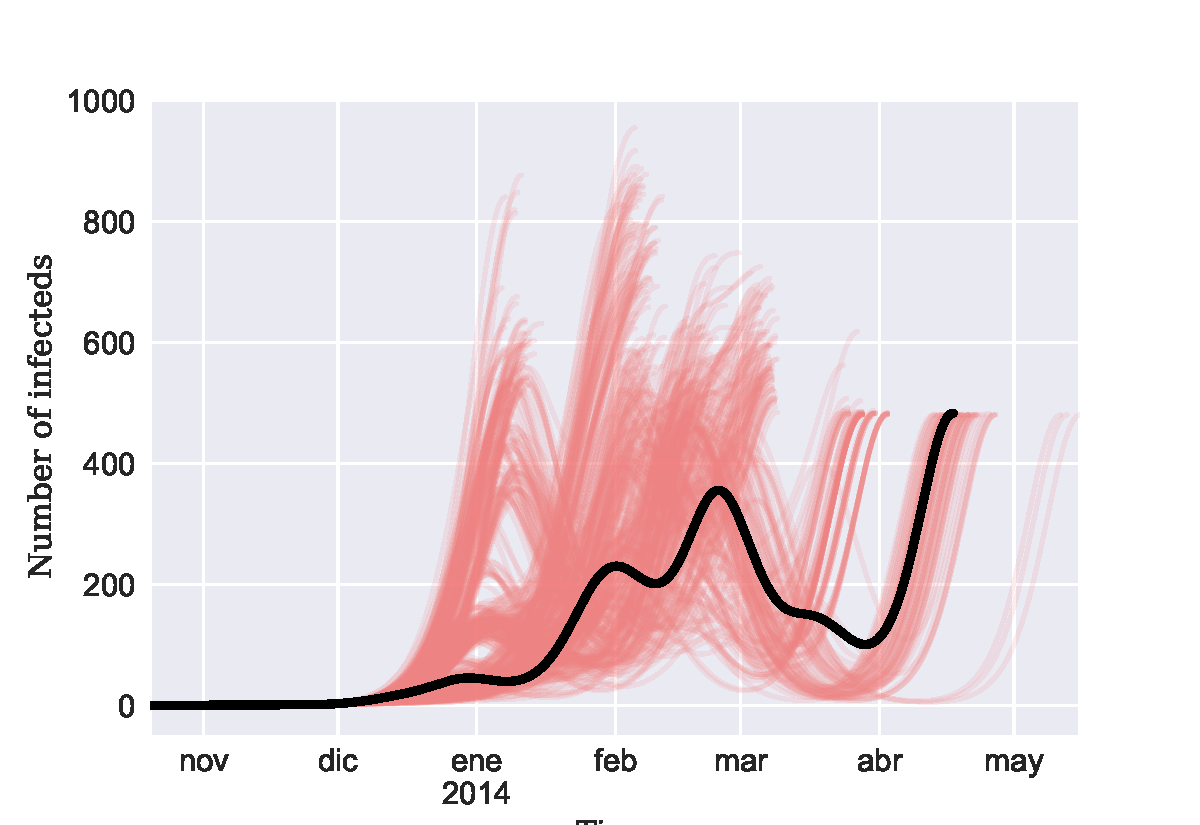
\includegraphics[scale=.30]{./scenario_A_2peak}
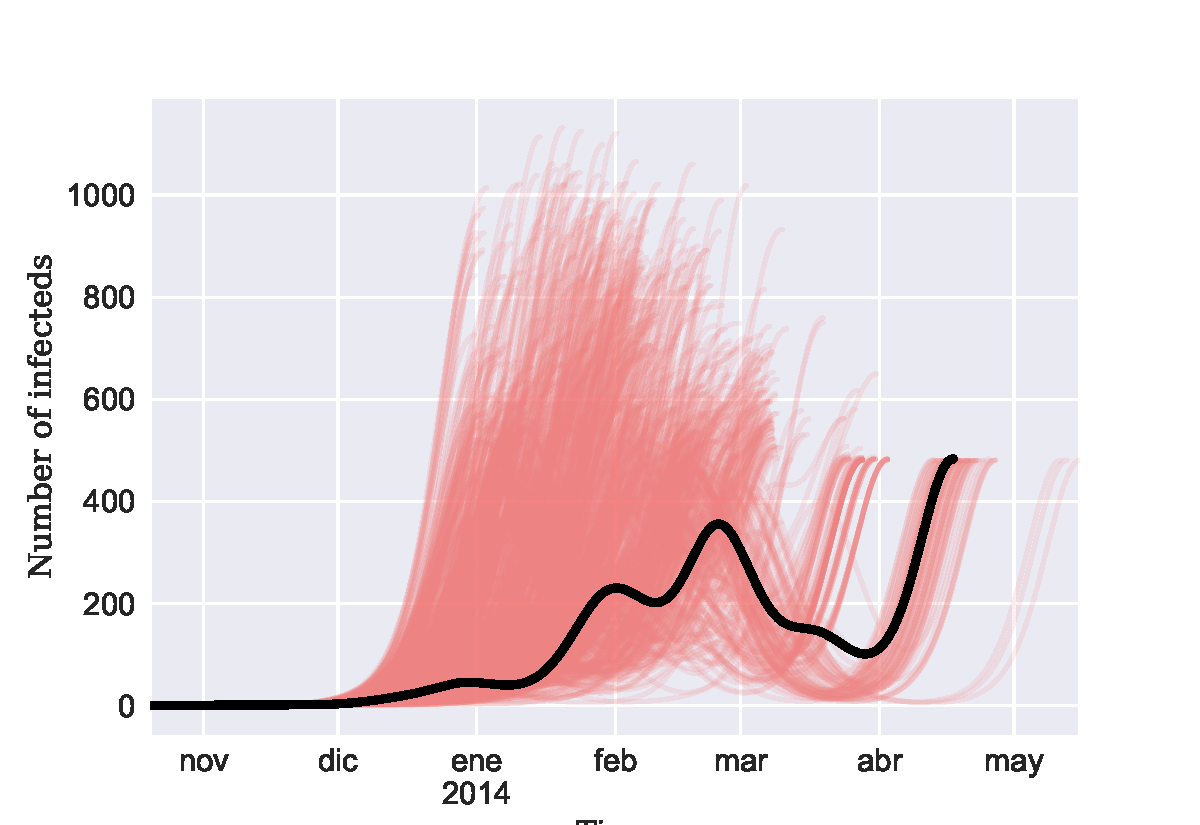
\includegraphics[scale=.30]{./scenario_D_2peak}
\caption{\small . (...)}
\label{fig:map-and-network}
\end{figure}
%
\vspace{2cm}
%
\begin{figure}[ht]
\centering
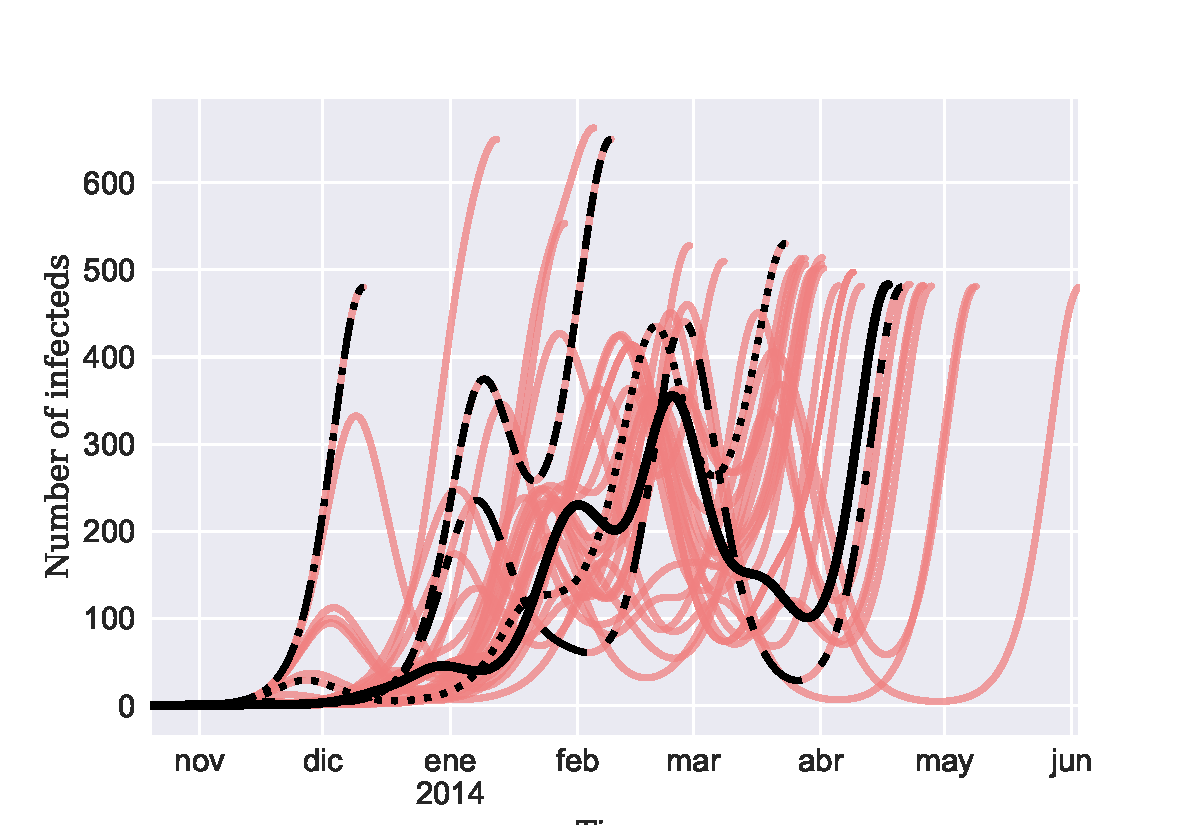
\includegraphics[scale=.35]{./scenario4_scenarioB-2}
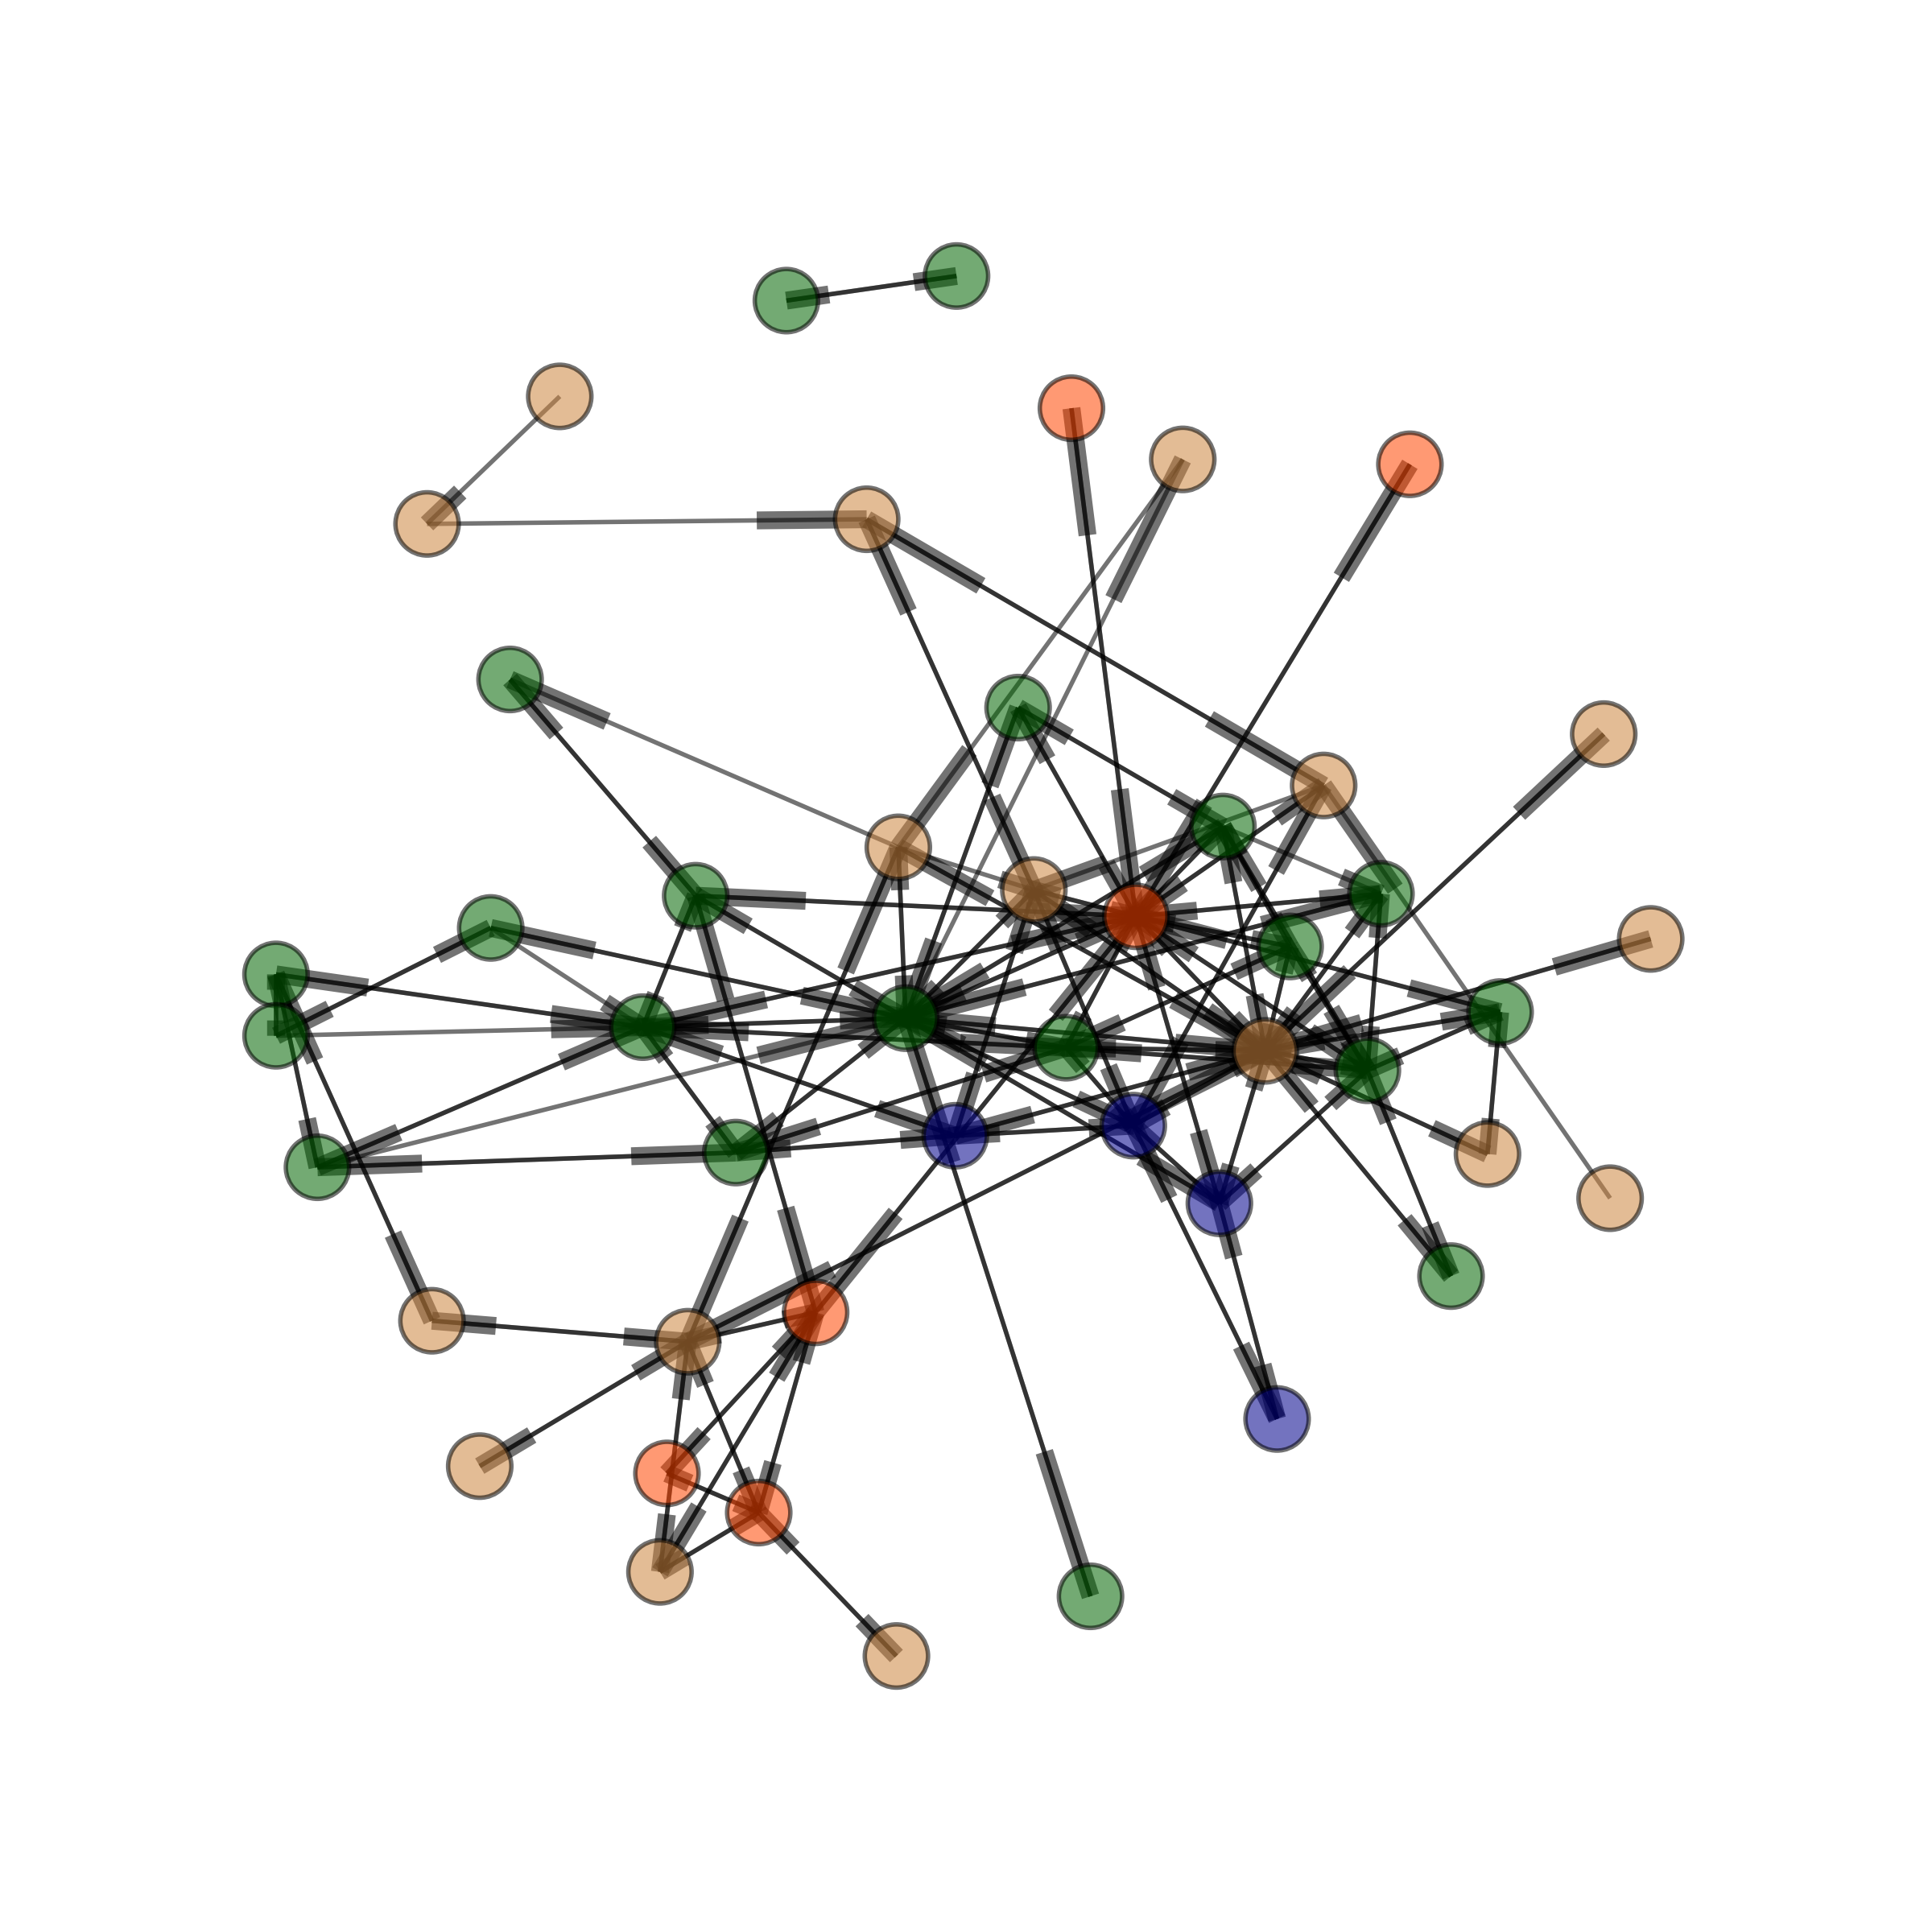
\includegraphics[scale=.30]{./graph_region3_colored} //
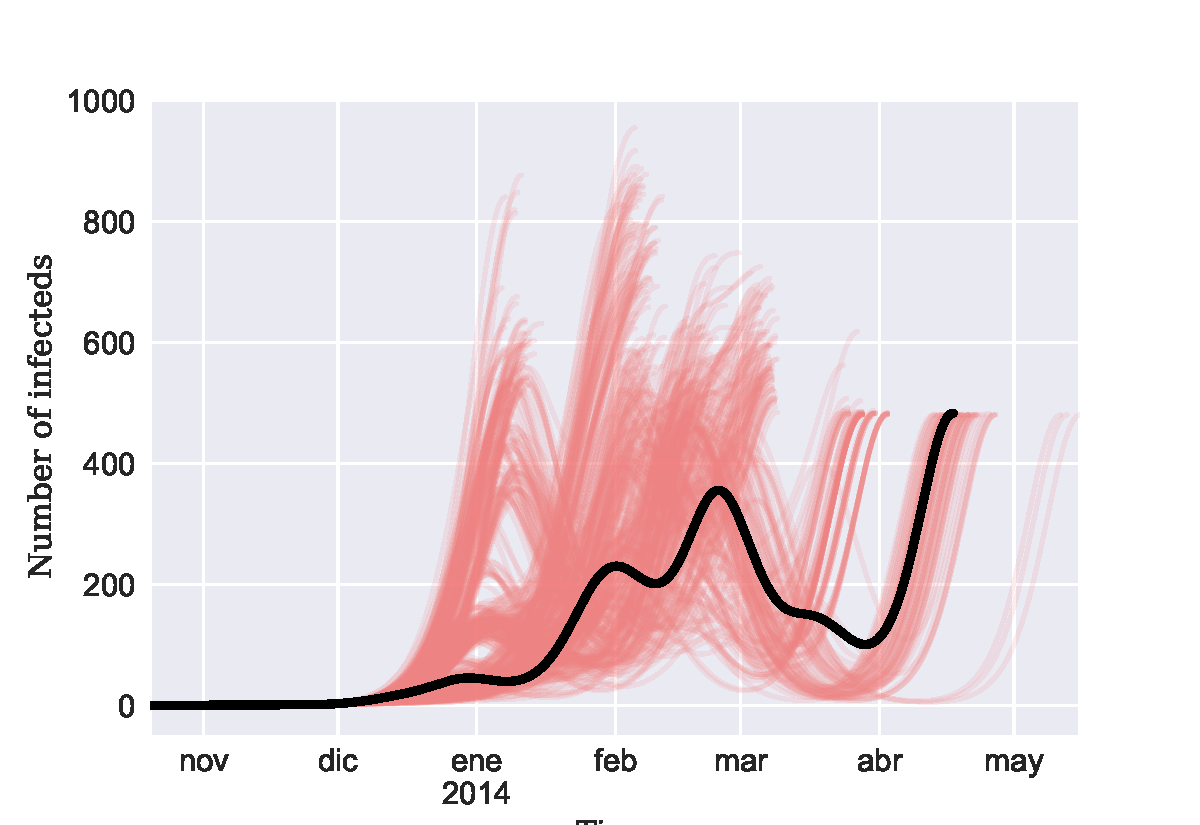
\includegraphics[scale=.30]{./scenario_A_2peak}
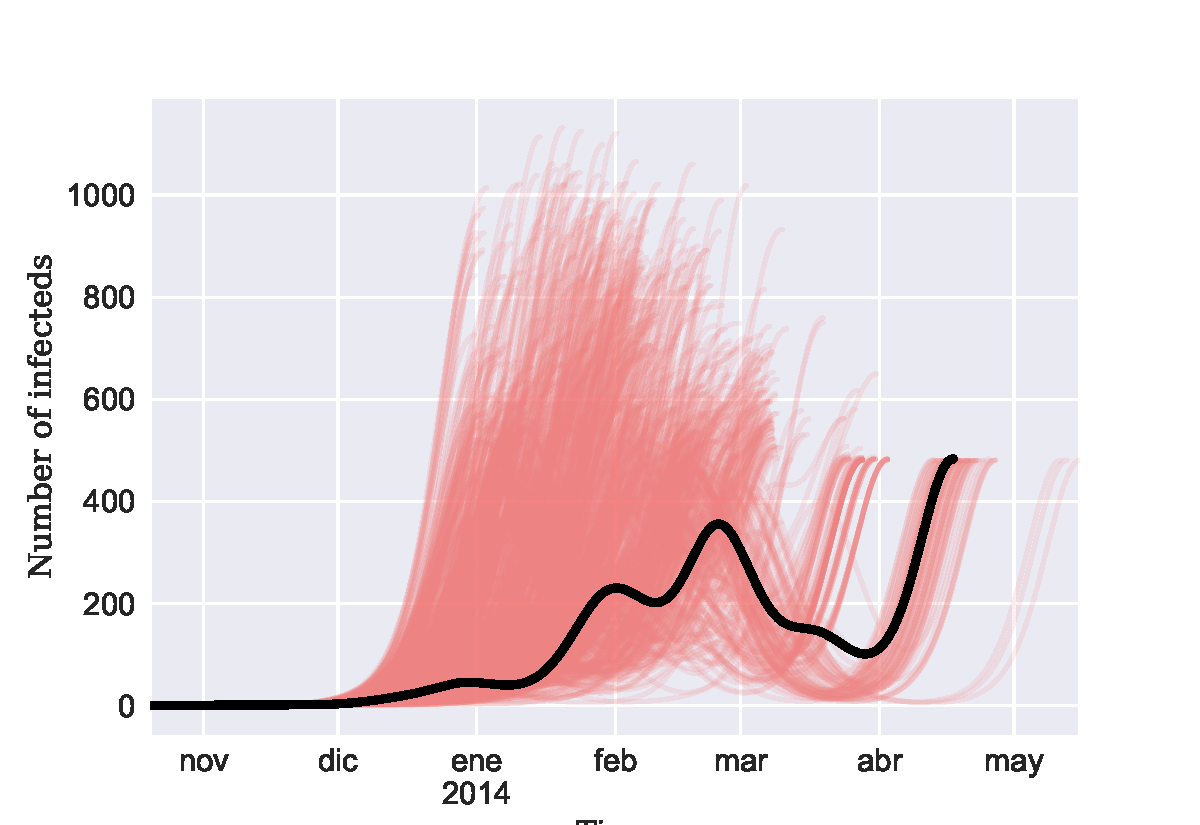
\includegraphics[scale=.30]{./scenario_D_2peak}
\caption{\small . (...)}
\label{fig:map-and-network}
\end{figure}


\end{document}
